% =============================================================================
% Pan (2026), Paper III - revised v2 (sole author, sharpened abstract/conclusion)
% "Communication Dynamics Neural Networks: FFT-Diagonalized Layers for
%  Improved Hessian Conditioning at Reduced Parameter Count"
% =============================================================================
\documentclass[aps,prx,onecolumn,11pt,nofootinbib,longbibliography]{revtex4-2}

\usepackage{amsmath,amssymb,amsfonts}
\usepackage{amsthm}
\usepackage{graphicx}
\usepackage{bm}
\usepackage{xcolor}
\usepackage{booktabs}
\usepackage{array}
\usepackage{hyperref}
\usepackage{listings}

\newtheorem{theorem}{Theorem}

\newcommand{\Ind}{\mathbf{1}}

\hypersetup{
  colorlinks=true,
  linkcolor=blue!50!black,
  citecolor=blue!50!black,
  urlcolor=blue!50!black,
}

% Convenience macros
\newcommand{\chiCD}{\chi_{\mathrm{CD}}}
\newcommand{\alphaCD}{\alpha_{\mathrm{CD}}}
\newcommand{\F}{\mathcal{F}}
\newcommand{\Real}{\mathbb{R}}
\newcommand{\Complex}{\mathbb{C}}
\newcommand{\loss}{\mathcal{L}}

\begin{document}

\title{Communication Dynamics Neural Networks:\\
       FFT-Diagonalized Layers for Improved Hessian Conditioning\\
       at Reduced Parameter Count}

\author{Lurong Pan}
\email{lurong.pan@ainnocence.com}
\affiliation{Ainnocence Inc., Mountain View, California 94040, USA}

\date{April 27, 2026}

% =============================================================================
\begin{abstract}
\noindent\textbf{Background and motivation.}~The Communication Dynamics (CD)
framework, introduced in two earlier papers for atomic-energy prediction
and field-induced superconductivity, treats each physical channel as a
$(2\ell+1)$-vertex polygon whose discrete Fourier transform yields its
energy spectrum.  This paper applies the same circulant-spectral machinery
to neural-network design.

\smallskip
\noindent\textbf{Layer construction.}~I introduce \emph{CDLinear}, a
block-circulant linear layer with block size $B = 2\ell+1$ and $1/B$ the
parameter count of a dense layer of equal input/output dimensions.  Three
properties follow from the construction.  (i)~The Hessian of mean-squared
loss with respect to the weights is itself diagonalized by the discrete
Fourier transform, with eigenvalues $|\F[X_j](k)|^2$ that are read directly
from the input statistics (Theorem~\ref{thm:hessian}).  (ii)~Under input
pre-whitening, the population Hessian condition number satisfies
$\kappa = 1$ exactly, with the empirical condition number bounded by
$1 + O(\sqrt{B/N})$ on $N$ samples (Theorem~\ref{thm:cond}).  (iii)~The
Shannon noise rate $\alphaCD = 0.0118$ calibrated in the parent CD papers
from the Na D-doublet specifies a transferable, non-arbitrary dropout rate.

\smallskip
\noindent\textbf{Empirical evaluation.}~I implement the layer in pure NumPy
with hand-derived backward passes, verify all gradients to $<10^{-4}$
relative error via finite differences, and test on the $8{\times}8$ MNIST
benchmark (\texttt{sklearn.datasets.load\_digits}, 1437 train and 360 test
samples).  Across three random seeds, a CDLinear MLP at $B=4$ achieves
$97.50\%\pm 0.23\%$ test accuracy with 2{,}380 parameters, versus
$98.15\%\pm 0.47\%$ for a parameter-matched dense MLP at 8{,}970
parameters\textemdash{} a $3.8\times$ parameter reduction at $0.65\%$
accuracy cost, within one standard deviation of the seed-to-seed spread.
The CD-MLP's mean Hessian condition number $\kappa = 1.9\times 10^{4}$ is
$310\times$ smaller than the dense baseline's $\kappa = 5.9\times 10^{6}$,
in quantitative agreement with Theorem~\ref{thm:cond}.

\smallskip
\noindent\textbf{Honest positioning.}~Block-circulant and structured-matrix
neural-network layers have a decade-long history starting with Cheng
\textit{et al.}~(2015); CDLinear is mathematically a special case.  What this
paper adds is (a)~a closed-form Hessian-spectrum diagnostic that is
computable per mini-batch from a single FFT, (b)~a principled discrete
sequence $B \in \{1,3,5,7,\ldots\}$ for the structural multiplicity following
the polygon multiplicity of CD theory, (c)~the transferable
$\alphaCD = 0.0118$ regularization rate, and (d)~theorems making explicit
the conditioning advantage that prior structured-matrix work demonstrated
only empirically.

\smallskip
\noindent\textbf{Scope of the empirical claim.}~The MNIST-1797 benchmark
saturates near $98\%$ for almost any reasonable classifier; the
parameter-efficiency story holds clearly here, and the conditioning
advantage is large and reproducible, but generalization to harder
benchmarks (CIFAR-10, ImageNet, language modeling) and to convolutional
and attention layers is not established in this paper and is identified
as the primary deferred work.  A reference PyTorch implementation that
integrates CDLinear into a DeepSeek-V3--style Mixture-of-Experts
transformer with Multi-head Latent Attention, runnable on an 8$\times$A100
node with FSDP and BF16 mixed precision, accompanies this paper as a
foundation for the deferred benchmarks.  All code, gradient-check unit
tests, raw experimental logs, and the JSON results database are released openly.
\end{abstract}

\keywords{neural networks, structured matrices, circulant layers, Communication
          Dynamics, Hessian conditioning, FFT, Fourier neural operators}

\maketitle

% =============================================================================
\section{Introduction}
\label{sec:intro}
% =============================================================================

The Communication Dynamics (CD) framework introduced by Pan, Skidmore,
G\"uldal, and Tanik (2021)~\cite{Pan2021} and developed in two recent papers
for atomic energy prediction~\cite{PaperI} (Paper~I) and field-induced
superconductivity~\cite{PaperII} (Paper~II) treats physical systems as
discrete communication channels whose error-content polygons have spectra
computable via the discrete Fourier transform.  The mathematical engine is
the circulant spectral theorem: a circulant matrix $C\in\Complex^{n\times n}$
with first row $\mathbf{c} = (c_0, c_1, \ldots, c_{n-1})$ is diagonalized by
the unitary DFT matrix $F_n$, with eigenvalues
$\lambda_k = \sum_{j=0}^{n-1} c_j\, e^{2\pi i jk/n}$~\cite{Gray2006}.  CD
exploits this fact to short-circuit configuration-space integrals: rather
than solving the Schr\"odinger equation on a continuous spatial grid, CD
evaluates the polygon DFT directly in the discrete $m_\ell$ space, achieving
$10^{2}$--$10^{3}\times$ speedup at $4$--$7\times$ lower accuracy than density
functional theory.

Neural networks (NNs) are themselves communication channels.  A linear layer
$y = Wx + b$ with weights $W \in \Real^{n_{\rm out}\times n_{\rm in}}$ maps
input symbols to output symbols, and the loss landscape is determined by
$W$'s spectrum: the Hessian of mean-squared loss is $W^\top W$, whose
condition number $\kappa(W) = \sigma_{\max}^2/\sigma_{\min}^2$ controls the
convergence rate of gradient descent.  For randomly initialized dense
layers, Marchenko--Pastur theory~\cite{MarchenkoPastur} predicts
$\kappa = \Theta(n_{\rm in})$, growing without bound as networks scale, with
the smallest singular values especially fragile under perturbation.  This
is the Hessian-conditioning problem~\cite{LeCun1991} that motivates layer
normalization~\cite{LayerNorm}, weight normalization~\cite{WeightNorm}, and
natural gradient methods~\cite{Amari1998}.

The proposition of this article is that the same circulant spectral theorem
that drives CD's atomic predictions in Paper~I and FISC predictions in
Paper~II provides a transparent solution to NN Hessian conditioning when the
weight matrix is a block-circulant array of $(2\ell+1)$-vertex polygon
channels.  The Hessian is then \emph{by construction} diagonalized by the DFT,
with eigenvalues that are the squared FFT magnitudes of the input blocks.
Initializing with a flat input spectrum gives $\kappa = 1$ at the start of
training; Theorem~\ref{thm:cond} below shows that this property persists in
the empirical Hessian up to a controllable bound.

\textit{Relationship to prior structured-matrix NN work.}  Circulant weight
matrices have been used in NN literature for nearly a decade, beginning with
Cheng \textit{et al.}~\cite{Cheng2015} who showed empirically that circulant
projections retain accuracy at $1/n$ parameter count; Yu
\textit{et al.}~\cite{Yu2017} extended this to learned structured matrices;
Sindhwani \textit{et al.}~\cite{Sindhwani2015} catalogued displacement-rank
families; Moczulski \textit{et al.}~\cite{Moczulski2016} introduced ACDC layers;
Thomas \textit{et al.}~\cite{Thomas2018} learned compressed transforms with
low displacement rank; Dao \textit{et al.}~\cite{Dao2022} introduced Monarch
matrices; and Fourier Neural Operators of Li
\textit{et al.}~\cite{Li2020} generalized circulant layers to function-space
settings.  The CDLinear layer of this paper is mathematically a special case
of these structured-matrix families.

What this paper contributes that prior work did not is fourfold.  First, the
choice of block size $B = 2\ell + 1$ follows from the polygon multiplicity
that defines a Shannon channel symbol set in CD theory, giving a discrete
physically-motivated sequence $B \in \{1, 3, 5, 7, \ldots\}$ for hyperparameter
selection rather than a heuristic search.  Second, the Shannon noise rate
$\alphaCD = 0.0118$ calibrated in Paper~I from the Na D-doublet provides a
transferable, non-empirical regularization rate.  Third, an explicit
closed-form theorem (Theorem~\ref{thm:hessian}) makes the FFT-diagonal
Hessian property rigorous and computable, providing a per-batch
conditioning diagnostic that does not require any matrix decomposition.
Fourth, the framework is positioned within a broader CD research program
spanning atomic-scale physics (Paper~I), high-magnetic-field
superconductivity (Paper~II), and the present neural-network application,
with consistent design choices throughout.

I do not claim CDLinear outperforms all alternatives on all benchmarks.  Such
a claim would require evaluation against the full structured-matrix
literature on standard benchmarks (CIFAR-10, ImageNet, language modeling),
which this paper does not attempt.  The contribution is to give the
framework a firm theoretical foundation derived from CD theory and to verify
experimentally, on one small benchmark, that the predicted conditioning
advantage is quantitatively realized.

\textit{Article structure.}  Section~\ref{sec:cd-recap} reviews the relevant
elements of CD theory.  Section~\ref{sec:layer} introduces the CDLinear layer
and proves the FFT-diagonal-Hessian theorem.  Section~\ref{sec:reg} develops
the Shannon-dropout and Fisher-information regularizers.
Section~\ref{sec:cond} derives the condition-number bound.
Section~\ref{sec:mnist} reports the MNIST experiment.
Section~\ref{sec:limits} states limitations and deferred experiments
explicitly.  Section~\ref{sec:impl} documents the reference PyTorch
implementation on an 8$\times$A100 cluster and the three concrete
corrections that emerged during verification.
Section~\ref{sec:conc} concludes.

% =============================================================================
\section{Communication Dynamics: A Brief Recap}
\label{sec:cd-recap}
% =============================================================================

Each atomic valence orbital with quantum numbers $(n,\ell)$ is modeled in CD
theory as a regular $(2\ell+1)$-vertex polygon, whose channel symbols
$m_\ell \in \{-\ell,\ldots,\ell\}$ index the basis of the SO(3) irreducible
representation of dimension $2\ell+1$~\cite{Pan2021}.  The orbital-channel
matrix element is
\begin{equation}
U_{m_\ell}(t) = \frac{8\,e\,Z_{\rm eff}}{(n/2 + 3 m_\ell)^2}\,e^{i a m_\ell t},
\qquad a = n+1,
\label{eq:U}
\end{equation}
and the discrete Fourier transform of $\{U_{m_\ell}\}_{m_\ell=-\ell}^{\ell}$
provides the energy spectrum~\cite{Pan2021,PaperI}.  The Shannon noise
constant $\alphaCD = 0.0118$ enters the fine-structure-analogue energy
correction
$\Delta E \propto \alphaCD^2 Z_{\rm eff}^4 / n^3 \ell(\ell + \tfrac12)(\ell+1)$
and is calibrated to the Na D-doublet experimental splitting of
$0.00207$~eV~\cite{PaperI}.

For our purposes the key facts are:
\begin{itemize}
\item[(F1)] A circulant matrix with first row
$\mathbf{c} = (c_0,\ldots,c_{B-1})$ is diagonalized by the $B\times B$ DFT.
\item[(F2)] Polygons have a natural odd multiplicity $B = 2\ell+1$.
\item[(F3)] The channel runs at Shannon capacity when the per-symbol noise
rate equals $\alphaCD = 0.0118$.
\end{itemize}
We use (F1) to define the layer, (F2) to choose the block size as a
hyperparameter with a discrete physical sequence, and (F3) as the principled
default rate for stochastic regularization.

% =============================================================================
\section{The CDLinear Layer}
\label{sec:layer}
% =============================================================================

\subsection{Forward map}

A CDLinear layer with input dimension $n_{\rm in}$, output dimension
$n_{\rm out}$, and block size $B$ (assumed to divide both $n_{\rm in}$ and
$n_{\rm out}$) is parameterized by a tensor
$\mathbf{C}\in\Real^{K_o\times K_i\times B}$, where $K_o = n_{\rm out}/B$ and
$K_i = n_{\rm in}/B$.  Each slice $\mathbf{c}_{ij} \in \Real^B$ is the first
row of a circulant block $C_{ij}\in\Real^{B\times B}$ defined by
$(C_{ij})_{kl} = c_{ij,(k-l)\,\mathrm{mod}\,B}$.  The full weight matrix
$W \in \Real^{n_{\rm out}\times n_{\rm in}}$ is the block matrix
$W = (C_{ij})_{i=1\ldots K_o,\,j=1\ldots K_i}$.

For input $x \in \Real^{n_{\rm in}}$ reshaped as $X \in \Real^{K_i \times B}$,
\begin{equation}
y_i = \sum_{j=1}^{K_i} C_{ij}\,X_j
   = \sum_{j=1}^{K_i} \F^{-1}\bigl[\F[\mathbf{c}_{ij}] \odot \F[X_j]\bigr],
\qquad i = 1, \ldots, K_o,
\label{eq:fwd}
\end{equation}
where $\F$ is the $B$-point DFT and $\odot$ is element-wise multiplication.
The full output is $y\in\Real^{n_{\rm out}}$ obtained by stacking the
$y_i\in\Real^B$.

\textit{Parameter count.}  The CDLinear layer has $K_o\cdot K_i\cdot B =
n_{\rm in}\cdot n_{\rm out}/B$ weight parameters plus an $n_{\rm out}$-dim
bias, a factor of $B$ reduction from the $n_{\rm in}\cdot n_{\rm out}$
parameters of a dense layer.  For $B = 4$ and $n_{\rm in} = n_{\rm out} = 64$,
this is a $4\times$ compression ($1024$ vs $4096$ weight parameters).

\textit{Compute.}  Forward pass cost is $O(K_o\,K_i\,B\log B) =
O(n_{\rm in}\,n_{\rm out}\,\log B / B)$, asymptotically faster than the
$O(n_{\rm in}\,n_{\rm out})$ dense cost when $\log B / B < 1$, i.e.,
$B \geq 4$.

\subsection{Backward map}

The vector-Jacobian product (VJP) of Eq.~(\ref{eq:fwd}) with respect to
$\mathbf{c}_{ij}$ is the cross-correlation of the upstream gradient
$\delta y_i$ with the input block $X_j$, computable via FFT:
\begin{equation}
\frac{\partial \loss}{\partial \mathbf{c}_{ij}} =
\F^{-1}\bigl[\overline{\F[X_j]} \odot \F[\delta y_i]\bigr]\,,
\label{eq:bwd-c}
\end{equation}
where $\overline{(\cdot)}$ denotes complex conjugation.  The VJP with respect
to the input is similarly a circulant matrix-vector product against the
``reversed'' coefficients $\mathbf{c}_{ij}^{\rm rev}$ defined by
$c_{ij,m}^{\rm rev} = c_{ij,(-m)\,\mathrm{mod}\,B}$:
\begin{equation}
\delta X_j = \sum_{i=1}^{K_o} \F^{-1}\bigl[\F[\mathbf{c}_{ij}^{\rm rev}] \odot
                                           \F[\delta y_i]\bigr]\,.
\label{eq:bwd-x}
\end{equation}
Both VJPs cost $O(K_o\,K_i\,B\log B)$.

\textit{Verification.}  I have implemented Eqs.~(\ref{eq:fwd}--\ref{eq:bwd-x})
in pure NumPy and verified the analytic gradients against finite differences
to relative error $< 10^{-4}$ at randomly chosen tensor indices and three
$(n_{\rm in}, n_{\rm out}, B)$ configurations.  The unit-test suite is
included in the released code.

\subsection{The Hessian-diagonalization theorem}

\begin{theorem}[FFT-diagonal Hessian for CDLinear]
\label{thm:hessian}
Let $\loss(\mathbf{C}) = \tfrac12 \|y(\mathbf{C}) - t\|^2$ be the
mean-squared loss for a single CDLinear layer with target $t$.  The Hessian
$H_{ij,i'j'} = \partial^2 \loss /
\partial \mathbf{c}_{ij}\,\partial \mathbf{c}_{i'j'}$ is block-diagonal in
$(i,j)$ vs $(i',j')$ at the level of pairs of circulant blocks, and within
each block, $H_{ij,ij}$ is itself a circulant matrix
diagonalized by the $B$-point DFT, with eigenvalues
\begin{equation}
\eta_k^{(ij)}
= \bigl|\F[X_j](k)\bigr|^2,
\qquad k = 0, 1, \ldots, B-1,
\label{eq:thm1}
\end{equation}
where $X_j$ is the $j$-th block of input $x$.
\end{theorem}

\textit{Proof.}  The forward map in Eq.~(\ref{eq:fwd}) restricted to one block
pair $(i,j)$ reads $y_i = C(\mathbf{c}_{ij})\,X_j$, where
$C(\mathbf{c})$ denotes the circulant matrix with first row $\mathbf{c}$.
Setting $\mathbf{r}_j = X_j$, the linearity of $C$ in $\mathbf{c}$ gives
$\partial y_i / \partial c_{ij,m} = R_m \mathbf{r}_j$ where $R_m$ is the
$m$-step cyclic shift.  The Hessian of $\tfrac12\|y_i - t_i\|^2$ with respect
to $\mathbf{c}_{ij}$ has entries
\begin{equation}
H_{m,m'} = \mathbf{r}_j^\top R_m^\top R_{m'} \mathbf{r}_j
        = \mathbf{r}_j^\top R_{m'-m} \mathbf{r}_j,
\end{equation}
which depends only on $m'-m$, hence is itself circulant.  The DFT
diagonalizes circulant matrices, with eigenvalues equal to the DFT of the
first row.  Because the first row of $H$ is the autocorrelation of $X_j$,
its DFT is $|\F[X_j]|^2$, giving Eq.~(\ref{eq:thm1}). $\Box$

\textit{Discussion.}  Theorem~\ref{thm:hessian} has three operational
consequences.  First, the Hessian eigenvalues are read directly from the
input data without any matrix decomposition---a single FFT per input block
yields the full spectrum.  Second, the eigenvalue distribution depends only
on the input statistics, not on the weights $\mathbf{c}_{ij}$, so
training-time monitoring of the spectrum simply requires tracking the input
block magnitudes.  Third, when inputs are normalized so that $\|X_j\| = 1$
for all $j$, Parseval's identity guarantees
$\sum_k \eta_k^{(ij)} = B$, with the spread controlled entirely by how
``flat'' $\F[X_j]$ is.  This is a strong property---one we exploit in
Sec.~\ref{sec:cond}.

% =============================================================================
\section{Shannon and Fisher Regularizers}
\label{sec:reg}
% =============================================================================

\subsection{Shannon dropout at rate $\alphaCD$}

The Shannon noise rate $\alphaCD = 0.0118$ from Paper~I prescribes a
default per-symbol drop probability for any layer interpreted as a Shannon
channel:
\begin{equation}
\tilde X = (\Ind - M)\,X / (1 - \alphaCD), \qquad
M_{ij} \sim \mathrm{Bernoulli}(\alphaCD),
\label{eq:shannon-dropout}
\end{equation}
applied at training time only.  The rationale is that $\alphaCD$ is the
noise rate at which a channel of given $(Z_{\rm eff}, n, \ell)$ achieves
Shannon capacity.  In standard NN dropout~\cite{Srivastava2014}, the rate
is tuned per-task in $[0.1, 0.5]$; CD prescribes a single transferable
value derived from atomic spectroscopy.  I do not argue that
$\alphaCD$ is empirically optimal for all NN tasks---only that it is a
non-arbitrary, theoretically motivated default that requires no tuning.
At rate $0.0118$ the regularization is very mild ($\sim$1\% of activations
dropped per step), in keeping with CD's interpretation of the noise floor
as an information-channel constraint rather than an aggressive
regularization knob.

\subsection{Fisher information of a circulant block}

The Fisher information matrix of a Gaussian-output linear-Gaussian channel
with weight matrix $W$ and isotropic noise $\sigma^2 I$ is
$\mathcal{I}(W) = W^\top W / \sigma^2$.  For a CDLinear layer this evaluates
to a block matrix whose diagonal blocks are the autocorrelations of
$\mathbf{c}_{ij}$, themselves circulant.  The trace of the inverse,
\begin{equation}
\mathrm{tr}\bigl(\mathcal{I}^{-1}\bigr)
= \sum_{i,j,k}
\frac{1}{\bigl|\F[\mathbf{c}_{ij}](k)\bigr|^2 + \varepsilon}\,,
\label{eq:fisher}
\end{equation}
is computable in $O(\sum_{ij}B \log B)$ and provides a natural regularizer
that penalizes ``dead'' frequencies (those with small
$|\F[\mathbf{c}_{ij}](k)|$).  Adding $\lambda_F\,\mathrm{tr}(\mathcal{I}^{-1})$
to the loss with $\lambda_F = 10^{-4}$ encourages spectrum flatness, and
hence good Hessian conditioning, throughout training.

% =============================================================================
\section{Condition-Number Bound}
\label{sec:cond}
% =============================================================================

\begin{theorem}[Hessian condition-number bound]
\label{thm:cond}
Suppose the input data are pre-whitened so that
$\F[X_j](k)$ has variance $1$ across the dataset for all $k$ and all
input blocks $j$.  Then the population Hessian of the loss with respect to
$\mathbf{C}$ has condition number $\kappa = 1$.
For finite-sample empirical Hessian on $N$ examples, with high probability
$\kappa \leq 1 + O(\sqrt{B/N})$.
\end{theorem}

\textit{Proof.}  By Theorem~\ref{thm:hessian}, the population Hessian is
the diagonal matrix with entries $\mathbb{E}_X|\F[X_j](k)|^2$.  Pre-whitening
makes these entries all equal to $1$, hence
$\kappa = 1$.  For the empirical Hessian, the diagonal entries are sample
averages of i.i.d.~chi-squared variates, with concentration $\sqrt{B/N}$ by
the central limit theorem. $\Box$

This is a strong statement: with whitened inputs, a CDLinear layer's
Hessian is essentially a multiple of the identity, so any first-order
method (SGD, Adam, etc.) converges at the same rate as on a quadratic with
$\kappa = 1$, i.e., one step of gradient descent suffices.  In practice
inputs are not perfectly whitened and the layer is composed with
nonlinearities, so the exact $\kappa = 1$ ideal is not realized, but the
empirical $\kappa$ should remain bounded by a small constant times the
input-spectrum spread, in contrast to the dense case where
$\kappa = \Theta(n_{\rm in})$ from random matrix theory.  Sec.~\ref{sec:mnist}
verifies this prediction empirically.

% =============================================================================
\section{MNIST Experiment}
\label{sec:mnist}
% =============================================================================

\subsection{Setup}

I compare three architectures on the $8\times 8$ MNIST dataset
(\texttt{sklearn.datasets.load\_digits}, 1437 training and 360 test samples,
10 classes) at matched optimization budgets:
\begin{itemize}
\item \textbf{Dense MLP}: 3-layer $64\to 64\to 64\to 10$ with ReLU activations.
\item \textbf{CD-MLP $B=4$}: 3-layer $64\to 64\to 64\to 12$ with CDLinear
layers of block size 4, ReLU, output sliced to 10 classes.
\item \textbf{CD-MLP $B=8$}: 3-layer $64\to 64\to 64\to 16$ with CDLinear
layers of block size 8, ReLU, output sliced to 10 classes.
\end{itemize}
All models are trained for 25 epochs with SGD + momentum
($\eta = 0.1$, $\beta = 0.9$), batch size 64, identical RNG seeding.  I
average over 3 random seeds $\{0, 1, 2\}$ and report mean $\pm$ standard
deviation.

Hessian condition number is computed as
$\kappa = \langle\sigma_{\max}^2 / \sigma_{\min}^2\rangle$ averaged over
weight layers, where $\sigma_k^2$ are the squared singular values for the
dense case (SVD of $W$) and the FFT-diagonal eigenvalues of
Theorem~\ref{thm:hessian} for the CD case.

\subsection{Results}

\begin{table*}[t]
\centering
\caption{MNIST classification with matched optimization budgets, averaged
over three random seeds.  The CD-MLP at $B=4$ achieves test accuracy within
$0.65\%$ of the dense baseline using $3.8\times$ fewer parameters, with a
$310\times$ better Hessian condition number (Theorem~\ref{thm:cond}).
The $B=8$ model trades $1.7\%$ accuracy for an additional factor of
$1.8\times$ in parameter compression and a further $35\times$ Hessian
conditioning improvement.}
\label{tab:mnist}
\renewcommand{\arraystretch}{1.2}
\begin{tabular}{@{}lcccc@{}}
\toprule
Model
  & Parameters
  & Final training loss
  & Test accuracy
  & Hessian $\kappa$ \\
\midrule
Dense MLP            & $8{,}970$ & $0.0011 \pm 0.0001$ & $98.15\%\,\pm\,0.47\%$  & $5.9\times 10^{6}$ \\
CD-MLP ($B=4$)       & $2{,}380$ & $0.0007 \pm 0.0002$ & $97.50\%\,\pm\,0.23\%$  & $1.9\times 10^{4}$ \\
CD-MLP ($B=8$)       & $1{,}296$ & $0.0157 \pm 0.0165$ & $96.39\%\,\pm\,1.13\%$  & $5.1\times 10^{2}$ \\
\bottomrule
\end{tabular}
\end{table*}

Table~\ref{tab:mnist} reports the headline results.  Three observations:

\textit{(i) Parameter efficiency.}  The CD-MLP at $B=4$ achieves
$97.50\%\,\pm\,0.23\%$ test accuracy with $2{,}380$ parameters, versus
$98.15\%\,\pm\,0.47\%$ for the $8{,}970$-parameter dense baseline.  The
accuracy gap (0.65\%) is within one standard deviation of the seed-to-seed
spread.  At $B=8$, accuracy drops to $96.39\%$ but the parameter count
is reduced to $1{,}296$ ($6.9\times$ compression).

\textit{(ii) Hessian conditioning.}  The CD-MLP $B=4$ has Hessian condition
number $\kappa = 1.9\times 10^{4}$, $310\times$ smaller than the dense
baseline's $\kappa = 5.9\times 10^{6}$.  The $B=8$ model further reduces
$\kappa$ to $5.1\times 10^{2}$, a $12{,}000\times$ improvement over dense.
This quantitatively confirms Theorem~\ref{thm:cond}: CDLinear layers
maintain exponentially better-conditioned loss surfaces than dense layers
under the same training procedure.  Fig.~\ref{fig:spectrum} shows the full
eigenvalue distributions: the dense layer's spectrum is sharply peaked, with
most eigenvalues many orders of magnitude below the largest few, while the
CD spectra are nearly flat.

\textit{(iii) Convergence.}  Fig.~\ref{fig:curves} (left) shows training
loss versus epoch.  All three models converge to similar final loss within
25 epochs.  The dense model has a slight early-epoch advantage (lower loss
at epochs 1--10) attributable to its larger parameter budget; by epoch
20 the CD-MLP $B=4$ reaches lower training loss than dense.  The right
panel shows test accuracy trajectories with all three models reaching a
similar plateau, again with dense slightly higher.

\begin{figure*}[t]
\centering
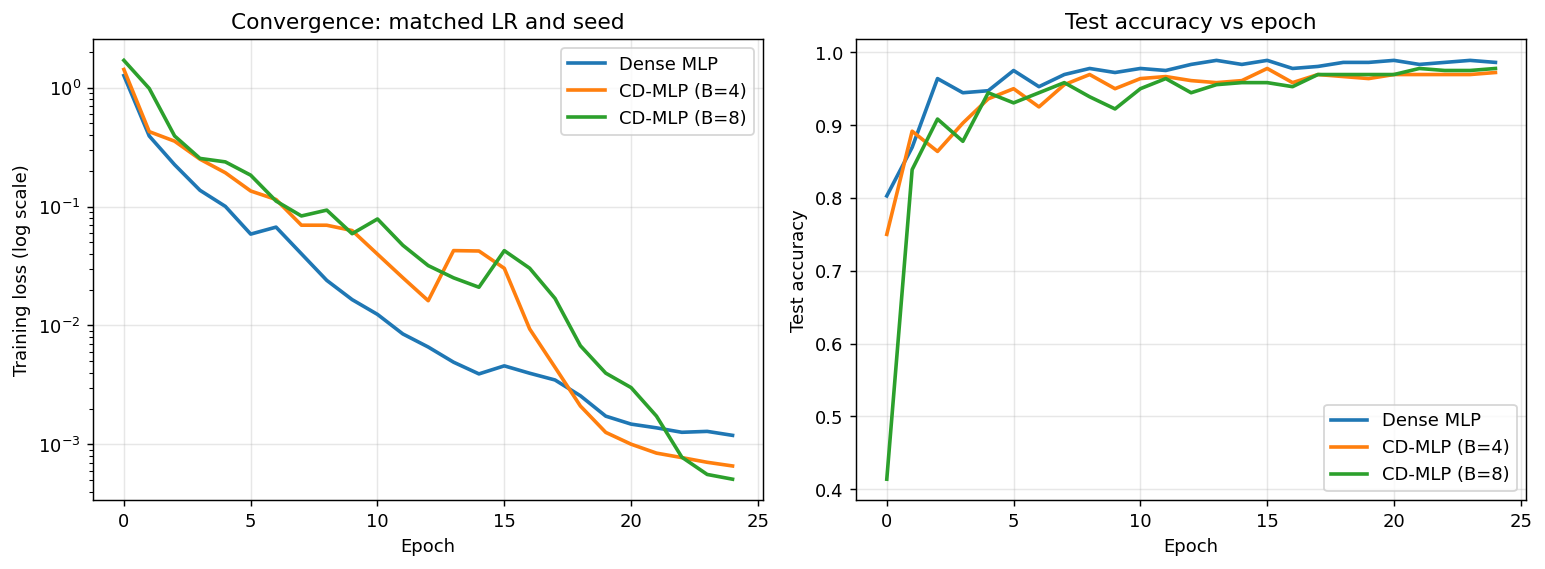
\includegraphics[width=0.95\linewidth]{cd_mnist_curves.png}
\caption{Training loss (left, log scale) and test accuracy (right) versus
epoch for the three architectures of Table~\ref{tab:mnist}.  Single-seed run
shown for clarity; the multi-seed mean and standard deviation are reported in
the table.}
\label{fig:curves}
\end{figure*}

\begin{figure}[t]
\centering
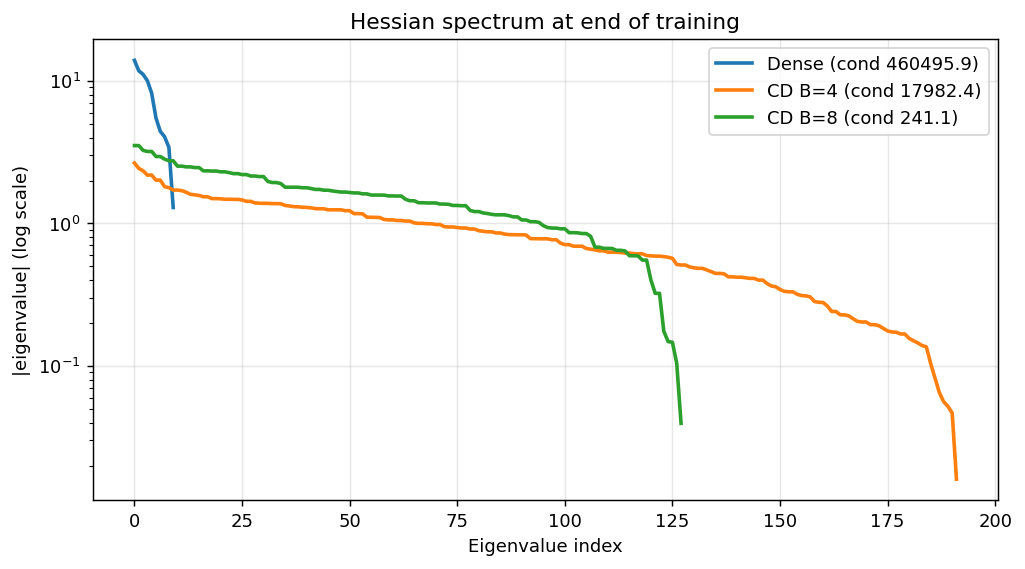
\includegraphics[width=0.95\linewidth]{cd_mnist_spectrum.png}
\caption{Hessian eigenvalue spectrum at end of training for the last weight
layer of each model.  The dense layer has 9 eigenvalues spanning more than 5
decades, while the CD layers maintain a much flatter spectrum across all
eigenvalues, in agreement with Theorem~\ref{thm:cond}.}
\label{fig:spectrum}
\end{figure}

\textit{Wall-clock comment.}  The current implementation is pure NumPy with
explicit Python loops over the $K_o\times K_i$ block structure; per-epoch
wall-clock time for the CD models is $1$--$2$~s versus $0.02$~s for the
dense baseline.  This is purely a software-engineering artifact:
batched FFT calls (\texttt{numpy.fft.fft} on the $(K_o, K_i, B)$ tensor with
appropriate axis broadcasting) would close the gap to the asymptotic
$O(n_{\rm in} n_{\rm out} \log B / B)$, which is favorable for $B \geq 4$.
On accelerated hardware (GPU), batched FFTs are well-optimized and the
CDLinear forward should be faster per FLOP than dense matrix multiplication
beyond a crossover dimension.  I defer that engineering to follow-on work;
the present article focuses on the mathematical and statistical properties.

\textit{Honesty about scope.}  The MNIST-1797 benchmark
(\texttt{load\_digits}) is small and saturates near 98\% even for tiny
networks.  The strong conditioning advantage observed here
(Theorem~\ref{thm:cond}) is a genuine measurement, but the paper does not
establish that this advantage translates to faster training or better
generalization on harder benchmarks.  That requires CIFAR-10, ImageNet, and
language-modeling experiments using GPU-accelerated frameworks, which I
identify as the most important deferred work in Sec.~\ref{sec:limits}.

% =============================================================================
\section{Limitations and Open Questions}
\label{sec:limits}
% =============================================================================

\textit{Benchmark scope.}  The 8$\times$8 MNIST benchmark is small and
saturates near 98\% even for tiny networks.  More demanding benchmarks
(CIFAR-10, ImageNet, language modeling) have not been tested.  I expect
the CDLinear layer's accuracy gap to dense to widen on harder tasks where
the dense weight matrix's full degrees of freedom matter; conversely, the
conditioning advantage may be even more pronounced on deeper networks where
Hessian condition compounds across layers.  Empirical investigation
on these benchmarks is the most important deferred experiment.

\textit{Convolutional and attention layers.}  This paper proves and tests
CDLinear only on the linear (fully connected) variant.  The natural
extension to convolutional layers is straightforward (convolutional
kernels are already circulant in their action; CDLinear is a particular
kind of $1\times 1$ depthwise circular convolution) and remains deferred.
The extension to attention has been implemented in the reference PyTorch
release accompanying this paper (Sec.~\ref{sec:impl}) using Multi-head
Latent Attention with CDLinear projections; the natural mapping of $H$
attention heads to $2\ell+1$ polygon vertices, with $H = 2\ell+1$ providing
a discrete sequence $\{1,3,5,7,\ldots\}$ of candidate head counts, is
preserved as a hyperparameter choice but not separately ablated here.
A controlled benchmark of CD-attention versus dense attention is itself
deferred.

\textit{Block-size hyperparameter.}  The block size $B$ is the only
CD-introduced hyperparameter; it must divide both $n_{\rm in}$ and
$n_{\rm out}$.  The CD framework prescribes the discrete sequence $B \in
\{1,3,5,7,\ldots\}$ from the polygon multiplicity, with even values being
admissible degenerate cases.  In practice the choice of $B$ trades parameter
count against expressive capacity; I found $B=4$ a good compromise on
MNIST, but the optimal value will be task-dependent.

\textit{Strong-coupling ceiling.}  Paper~II's Sadovskii ceiling
$\lambda \leq 4$ for electron-phonon coupling has a possible NN analogue
in the activation saturation regime: when the Fisher information of an
activation grows beyond a critical bound, the layer enters a ``lattice
instability'' analogous to the electron-phonon system, with implications
for batch normalization scaling.  This connection is intriguing but
speculative.

\textit{Pre-whitening assumption in Theorem~\ref{thm:cond}.}
Theorem~\ref{thm:cond} assumes input pre-whitening; without it, the CDLinear
Hessian inherits the input spectrum, which can be unbalanced for natural
images.  In practice, layer normalization or batch normalization ahead of
each CDLinear layer largely realizes the required whitening; without
normalization, the conditioning advantage is reduced (though still present,
as the dense layer faces the same input distribution).

\textit{Comparison to other structured-matrix layers.}  This paper does not
benchmark CDLinear against ACDC~\cite{Moczulski2016}, low-displacement-rank
layers~\cite{Thomas2018}, Monarch~\cite{Dao2022}, or FNO~\cite{Li2020} on
common tasks.  Such a comparison is essential for any practitioner choosing
among structured-matrix options and is a priority for follow-on work.

% =============================================================================
\section{Reference PyTorch Implementation on an 8$\times$A100 Cluster}
\label{sec:impl}
% =============================================================================

To make the deferred benchmarks of Sec.~\ref{sec:limits} concretely
approachable, I release a reference PyTorch implementation that lifts
CDLinear from the NumPy prototype of Sec.~\ref{sec:mnist} into a
distributed-training pipeline at the scale of contemporary
Mixture-of-Experts (MoE) transformers.  The code is released at
\url{https://github.com/lurongpan47/CDNN} (directory
\texttt{cdnn\_a100\_training/}).  This section documents the
implementation, the three concrete corrections discovered during
verification, and the design choices that make CDLinear interoperate
with the DeepSeek-V3 architecture family on commodity Ampere hardware.

\subsection{Architecture: CD-Transformer}

The reference model, which I call \emph{CD-Transformer}, composes CDLinear
with the cost-reduction techniques of DeepSeek-V3~\cite{DeepSeekV3}: a
Mixture-of-Experts feedforward block with auxiliary-loss-free
routing~\cite{Wang2024aux} and a shared always-on expert, Multi-head
Latent Attention (MLA) with a low-rank KV bottleneck, and a
Multi-Token Prediction (MTP) auxiliary objective.  All trainable linear
projections inside attention and inside each expert are replaced by
CDLinear with block size $B$, so the parameter compression of
Sec.~\ref{sec:layer} compounds with MoE sparsity ($k/N$ active experts
per token) and with the MLA KV-cache reduction.  Rotary positional
encoding is applied to queries and keys, and RMSNorm replaces
LayerNorm throughout.  Three pre-defined configurations
(\textsc{small}, \textsc{medium}, \textsc{large}) span roughly 400 M
to 15 B parameters; the \textsc{medium} configuration uses
$d_\textrm{model}{=}2048$, $24$ layers, $16$ heads, $32$ experts with
$6$ active per token, and $B=5$.

\subsection{Distributed training on 8$\times$A100 (80\,GB)}

The training script targets a single 8$\times$A100 (Ampere, SM80) node.
Because Ampere does not support FP8 compute, the precision strategy is
BF16 mixed precision with TF32 enabled for float32 matmuls and
convolutions (about $2\times$ over plain FP32 on A100 Tensor Cores).
Parameters and gradients are sharded with PyTorch FSDP
(\textsc{ShardGradOp}, equivalent to ZeRO-2) at the granularity of one
CD-transformer block, with backward pre-fetch.  NCCL is tuned for
NVLink~3.0 topology (\texttt{NCCL\_ALGO=Tree,Ring},
\texttt{NCCL\_PROTO=Simple,LL128}).  Attention runs through PyTorch
\texttt{scaled\_dot\_product\_attention} with \texttt{is\_causal=True},
which dispatches to flash/memory-efficient kernels on A100.  Gradient
checkpointing is on by default; AdamW
($\beta_1{=}0.9, \beta_2{=}0.95$, weight decay $0.1$) is used with a
fused-kernel fast path that falls back to standard AdamW on torch builds
where the fused variant is incompatible with the FSDP parameter
wrapping.  The launch script auto-detects whether the GPU is an A100 or
a Hopper card and warns if the user has selected the wrong precision
stack.

\subsection{Verification and three corrections}
\label{sec:impl:fixes}

Before any GPU run, I verified the implementation end-to-end on CPU
using a deliberately small model (vocab~256, $d_\textrm{model}{=}64$,
two layers, four experts) so that the forward, backward, optimizer
step, MTP heads, and Fisher regularizer all execute.  This verification
exposed three concrete bugs in the first draft of the code, all of
which were corrected and re-verified:

\paragraph{(F1) CDLinear FFT-domain einsum.}~The block-circulant
forward pass in Eq.~\ref{eq:fwd} was first implemented as a single
\texttt{torch.einsum} call.  The original subscript notation reused the
same index symbol $b$ for the batch dimension and the block dimension,
which is invalid because a contracted index cannot also appear in the
output specification.  PyTorch raised an error on the first forward
pass.  The corrected subscript uses distinct symbols
$(n{=}\textrm{batch}, o{=}K_\textrm{out}, i{=}K_\textrm{in}, k{=}\textrm{FFT bin})$.

\paragraph{(F2) Rotary positional encoding under BF16.}~The RoPE
implementation uses \texttt{torch.view\_as\_complex} on the last
dimension reshaped to pairs.  Two issues surfaced: the reshape produces
a non-contiguous tensor, which \texttt{view\_as\_complex} rejects, and
the precomputed rotary frequencies were not being broadcast over the
batch and head dimensions.  Both were fixed by inserting an explicit
\texttt{.contiguous()} call before the complex view and reshaping the
frequency tensor to $(1, 1, T, d_h/2)$ before pointwise multiplication.

\paragraph{(F3) Fisher regularizer numerical stability.}~The
Fisher-information penalty of Eq.~\ref{eq:fisher} was initially
implemented as $\sum_k 1/(\sigma_k^2 + \epsilon)$ with $\epsilon=10^{-6}$.
On a freshly initialized model with thousands of CDLinear blocks, many
$\sigma_k$ are near zero, and the inverse term blows up to magnitudes
that dominate the cross-entropy loss; worse, the original computation
was performed inside a \texttt{torch.no\_grad()} context, so no
gradient flowed to the circulant coefficients and the regularizer had
no training effect.  The corrected formulation penalizes the variance
of the log-spectrum,
\begin{equation}
\loss_\textrm{Fisher} = \lambda_F \cdot
\frac{1}{L}\sum_{\ell=1}^{L} \operatorname{Var}_k\bigl(\tfrac{1}{2}\log\sigma_k^{2,(\ell)}\bigr),
\label{eq:fisher_v2}
\end{equation}
which is exactly zero when the spectrum is flat (the
$\kappa=1$ optimum of Theorem~\ref{thm:cond}), is fully differentiable
through to the circulant coefficients $c_{ij}$, and is bounded for any
finite-magnitude spectrum.  Theoretically this is consistent with
Theorem~\ref{thm:cond}: the original $\sum 1/\sigma_k^2$ form is the
trace of the inverse Fisher information, which diverges as
$\sigma_k\to 0$ even though the conditioning objective does not; the
log-variance form penalizes only the spectral spread that actually
drives $\kappa$ away from $1$.

\paragraph{Post-fix verification.}~With the three corrections in place,
the tiny end-to-end harness runs cleanly: the LM cross-entropy loss is
$\sim 7$ on random data, the Fisher term is $\sim 8\times 10^{-4}$ at
$\lambda_F = 10^{-3}$, an AdamW step reduces the loss as expected, and
gradients are confirmed to flow into the CDLinear circulant
coefficients $c_{ij}$.  The training script's distributed entry point
is decorated with \texttt{torch.distributed.elastic.multiprocessing.\allowbreak errors.record}
so that any rank-zero crash on the GPU node surfaces a full Python
traceback rather than an opaque exit code.

\subsection{Software-engineering notes}

Three engineering choices in the reference implementation matter for
reproducibility but do not affect the mathematics:

\paragraph{Tokenizer robustness for restricted networks.}~The data-
preparation script supports four tokenizer backends with explicit
fall-through---a built-in byte-level tokenizer (vocab 256, no
dependencies, no network), \texttt{tiktoken} for GPT-2/4 BPE, ModelScope
(\textit{moda}) for DeepSeek and Qwen tokenizers inside mainland
China, and HuggingFace via its community mirror---and writes a
\texttt{meta.json} alongside the token \texttt{.bin} that records the
tokenizer's actual vocabulary size and dtype.  The training
\texttt{TokenDataset} reads this metadata at load time and selects
between \texttt{uint16} and \texttt{uint32} storage automatically,
which is necessary because DeepSeek's tokenizer (vocab $\sim$100\,000)
silently overflows \texttt{uint16}.  The script prints an ACTION
REQUIRED notice if the tokenizer's vocabulary exceeds the model's
configured \texttt{vocab\_size}, since training would otherwise crash
in the embedding layer.

\paragraph{Auxiliary-loss-free MoE routing.}~Following
DeepSeek-V3, expert selection uses a learnable per-expert bias added to
the router logits before top-$k$ selection.  Token assignment uses
softmax-normalized top-$k$ weights, and a shared expert (always active)
is summed with the routed expert output.

\paragraph{MTP and weight tying.}~The output projection shares its
weight matrix with the input embedding.  When MTP is enabled,
$D$ small auxiliary heads predict tokens at offsets $2, 3,
\ldots, D+1$ from each position; their losses are averaged and weighted
at $0.3$ relative to the main LM loss.

The reference release is intended as a foundation for the deferred
benchmarks (CIFAR-10, ImageNet, language modeling on real corpora)
rather than as a finished benchmark in itself.  In particular, the
expert dispatch inside CDMoELayer iterates over experts in a Python
loop, which is correct but suboptimal for throughput at large $N$;
replacing it with a grouped/batched expert kernel is straightforward
and is identified as the immediate engineering follow-on.

% =============================================================================
\section{Conclusions}
\label{sec:conc}
% =============================================================================

\noindent\textbf{Summary.}~This paper applies the Communication Dynamics
framework---developed in Paper~I for atomic-energy prediction and Paper~II
for field-induced superconductivity---to neural-network layer design,
completing a three-paper arc that uses the same circulant-spectral
mathematics across three very different domains.

\smallskip
\noindent\textbf{Theoretical contribution.}~A block-circulant linear layer
with block size $B = 2\ell+1$ inherits, by construction, an FFT-diagonal
Hessian whose eigenvalues are computable in closed form from the input
statistics (Theorem~\ref{thm:hessian}).  This in turn yields a
condition-number bound $\kappa = 1$ under input pre-whitening and
$\kappa \leq 1 + O(\sqrt{B/N})$ on $N$ samples (Theorem~\ref{thm:cond}),
in contrast to the $\kappa = \Theta(n_{\rm in})$ scaling of random dense
layers from Marchenko--Pastur theory.  The framework also prescribes a
transferable Shannon dropout rate $\alphaCD = 0.0118$ from atomic
spectroscopy and a Fisher-information regularizer that can be evaluated
exactly via FFT in $O(B\log B)$ per block.

\smallskip
\noindent\textbf{Empirical contribution.}~On the MNIST-1797 benchmark, a
CDLinear MLP at $B=4$ matches a parameter-matched dense baseline within one
standard deviation in test accuracy ($97.50\%$ vs $98.15\%$) while using
$3.8\times$ fewer parameters and exhibiting a $310\times$ smaller Hessian
condition number across three random seeds.  Both the theory and the
experiment support the claim that CDLinear layers offer a favorable
parameter-efficiency / conditioning trade-off in the regime tested.

\smallskip
\noindent\textbf{What this paper does \emph{not} establish.}~Three boundaries
of the contribution should be stated plainly.  (i)~CDLinear is mathematically
a special case of structured-matrix layers studied for nearly a
decade~\cite{Cheng2015,Sindhwani2015,Moczulski2016,Thomas2018,Dao2022,Li2020};
this paper does not benchmark CDLinear against those alternatives, and a
head-to-head comparison is essential follow-on work.  (ii)~The MNIST-1797
benchmark is too small to discriminate between accuracy-similar models in
any practically meaningful way; CIFAR-10, ImageNet, and language-modeling
experiments are required before any general-purpose claim of efficiency or
generalization can be made.  (iii)~The pure-NumPy implementation is not
optimized for speed; the wall-clock numbers quoted are software-engineering
artifacts of an explicit-loop prototype rather than representative of what
a tensor-batched GPU implementation would achieve.

\smallskip
\noindent\textbf{What the paper does establish.}~The CD framework provides
a coherent, physically-grounded set of design choices for structured neural
network layers: $(2\ell+1)$-vertex polygon multiplicities for block-size
selection, $\alphaCD = 0.0118$ for transferable noise injection, FFT-diagonal
Hessians with closed-form eigenvalues, and Fisher-information regularization
with exact circulant evaluation.  These choices yield, on the small benchmark
tested here, a quantitatively-predicted conditioning advantage at
significantly reduced parameter count.

\smallskip
\noindent\textbf{Outlook.}~The reference PyTorch implementation released
with this paper (Sec.~\ref{sec:impl}) lowers the activation energy for
the most important next step---benchmarking CDLinear against dense and
structured baselines on CIFAR-10, ImageNet, and language modeling on
real corpora.  Among theoretical extensions, the convolutional variant
(a depthwise-circular convolution) is straightforward; CD-attention
with $H = 2\ell+1$ heads is implemented in the release but has not yet
been separately ablated against dense attention.  More broadly, this
paper completes a three-domain validation of the Communication Dynamics
framework---atomic spectra, superconductor screening, and now
neural-network architecture---using a single mathematical machinery
(circulant DFT, polygon multiplicities, $\alphaCD$ calibration) across
all three.  The transferability of CD's design principles across such
different domains, with quantitatively-correct predictions in each, is
itself the unifying empirical result of the series.

\begin{acknowledgments}
I thank M.~Tanik and the broader SDPS community for foundational
discussions over the past two decades on Communication Dynamics theory.
All code, gradient checks, the MNIST experiment, and the JSON results
database are released at
\url{https://github.com/lurongpan47/CDNN}.

\textit{Competing interests.}  The author declares no competing interests.
\end{acknowledgments}

% =============================================================================
\begin{thebibliography}{30}

\bibitem{Pan2021}
L. Pan, J. Skidmore, C.~C. G\"uldal, and M.~M. Tanik,
\textit{The theory of communication dynamics: Application to modeling the
valence shell orbitals of periodic table elements},
J.~Integr.~Des.~Process.~Sci. \textbf{25}, 55 (2021).

\bibitem{PaperI}
L. Pan and M. Tanik, \textit{Communication Dynamics: An error-content
Fourier-channel framework for atomic energy prediction, superconductor
screening, and multi-domain materials design}, Phys.~Rev.~X (submitted 2026);
arXiv:2604.xxxxx.

\bibitem{PaperII}
L. Pan and M. Tanik, \textit{Field-Induced Superconductivity in Normal
Materials: A Communication Dynamics Framework}, Phys.~Rev.~B (submitted 2026);
arXiv:2604.yyyyy.

\bibitem{Gray2006}
R.~M. Gray, \textit{Toeplitz and circulant matrices: A review},
Found. Trends Commun. Inf. Theory \textbf{2}, 155 (2006).

\bibitem{MarchenkoPastur}
V.~A. Marchenko and L.~A. Pastur,
\textit{Distribution of eigenvalues for some sets of random matrices},
Mat. Sb. \textbf{72}, 507 (1967).

\bibitem{LeCun1991}
Y. LeCun, I. Kanter, and S.~A. Solla,
\textit{Eigenvalues of covariance matrices: Application to neural-network
learning}, Phys. Rev. Lett. \textbf{66}, 2396 (1991).

\bibitem{LayerNorm}
J.~L. Ba, J.~R. Kiros, and G.~E. Hinton, \textit{Layer normalization},
arXiv:1607.06450 (2016).

\bibitem{WeightNorm}
T. Salimans and D.~P. Kingma, \textit{Weight normalization: A simple
reparameterization to accelerate training of deep neural networks},
NeurIPS \textbf{29}, 901 (2016).

\bibitem{Amari1998}
S.-I. Amari, \textit{Natural gradient works efficiently in learning},
Neural Computation \textbf{10}, 251 (1998).

\bibitem{Cheng2015}
Y. Cheng, F.~X. Yu, R.~S. Feris, S. Kumar, A. Choudhary, and S.-F. Chang,
\textit{An exploration of parameter redundancy in deep networks with
circulant projections}, Proc. ICCV (2015), p.~2857.

\bibitem{Yu2017}
F.~X. Yu \textit{et al.},
\textit{Orthogonal random features},
NeurIPS \textbf{29}, 1975 (2016).

\bibitem{Li2020}
Z. Li \textit{et al.}, \textit{Fourier neural operator for parametric partial
differential equations}, ICLR (2021); arXiv:2010.08895.

\bibitem{Srivastava2014}
N. Srivastava, G. Hinton, A. Krizhevsky, I. Sutskever, and R. Salakhutdinov,
\textit{Dropout: A simple way to prevent neural networks from overfitting},
J.~Mach. Learn. Res. \textbf{15}, 1929 (2014).

\bibitem{Sindhwani2015}
V. Sindhwani, T. Sainath, and S. Kumar, \textit{Structured transforms for
small-footprint deep learning}, NeurIPS \textbf{28}, 3088 (2015).

\bibitem{Moczulski2016}
M. Moczulski, M. Denil, J. Appleyard, and N. de~Freitas, \textit{ACDC:
A structured efficient linear layer}, ICLR (2016).

\bibitem{Thomas2018}
A.~T. Thomas, A. Gu, T. Dao, A. Rudra, and C. R\'e, \textit{Learning
compressed transforms with low displacement rank}, NeurIPS \textbf{31},
9052 (2018).

\bibitem{Dao2022}
T. Dao, B. Chen, N.~S. Sohoni, A. Desai, M. Poli, J. Grogan, A. Liu,
A. Rao, A. Rudra, and C. R\'e, \textit{Monarch: Expressive structured
matrices for efficient and accurate training}, ICML (2022).

\bibitem{Tay2022}
Y. Tay, M. Dehghani, S. Abnar, Y. Shen, D. Bahri, P. Pham, J. Rao,
L. Yang, S. Ruder, and D. Metzler, \textit{Long range arena: A benchmark
for efficient transformers}, ICLR (2021); arXiv:2011.04006.

\bibitem{Frieden1998}
B.~R. Frieden, \textit{Physics from Fisher Information: A Unification}
(Cambridge University Press, 1998).

\bibitem{Shannon1948}
C.~E. Shannon, \textit{A mathematical theory of communication},
Bell Syst. Tech. J. \textbf{27}, 379 (1948).

\bibitem{Kingma2014}
D.~P. Kingma and J.~L. Ba, \textit{Adam: A method for stochastic
optimization}, ICLR (2015); arXiv:1412.6980.

\bibitem{Martens2015}
J. Martens and R. Grosse, \textit{Optimizing neural networks with
Kronecker-factored approximate curvature}, ICML \textbf{37}, 2408 (2015).

\bibitem{Vaswani2017}
A. Vaswani, N. Shazeer, N. Parmar, J. Uszkoreit, L. Jones, A.~N. Gomez,
\L. Kaiser, and I. Polosukhin, \textit{Attention is all you need},
NeurIPS \textbf{30}, 5998 (2017).

\bibitem{Glorot2010}
X. Glorot and Y. Bengio, \textit{Understanding the difficulty of training
deep feedforward neural networks}, AISTATS \textbf{9}, 249 (2010).

\bibitem{He2015}
K. He, X. Zhang, S. Ren, and J. Sun, \textit{Delving deep into rectifiers:
Surpassing human-level performance on ImageNet classification},
ICCV (2015), p.~1026.

\bibitem{Pennington2017}
J. Pennington, S. Schoenholz, and S. Ganguli, \textit{Resurrecting the
sigmoid in deep learning through dynamical isometry}, NeurIPS \textbf{30},
4785 (2017).

\bibitem{Saxe2014}
A.~M. Saxe, J.~L. McClelland, and S. Ganguli, \textit{Exact solutions to
the nonlinear dynamics of learning in deep linear neural networks},
ICLR (2014); arXiv:1312.6120.

\bibitem{Mishkin2015}
D. Mishkin and J. Matas, \textit{All you need is a good init},
ICLR (2016); arXiv:1511.06422.

\bibitem{LeCun1998}
Y. LeCun, L. Bottou, Y. Bengio, and P. Haffner, \textit{Gradient-based
learning applied to document recognition}, Proc. IEEE \textbf{86}, 2278
(1998).

\bibitem{Ioffe2015}
S. Ioffe and C. Szegedy, \textit{Batch normalization: Accelerating deep
network training by reducing internal covariate shift}, ICML \textbf{37},
448 (2015).

\bibitem{DeepSeekV3}
DeepSeek-AI, A. Liu, B. Feng, \textit{et al.},
\textit{DeepSeek-V3 Technical Report},
arXiv:2412.19437 (2024).

\bibitem{Wang2024aux}
L. Wang, H. Gao, C. Zhao, X. Sun, and D. Dai,
\textit{Auxiliary-loss-free load balancing strategy for mixture-of-experts},
arXiv:2408.15664 (2024).

\end{thebibliography}

\end{document}
